\let\negmedspace\undefined
\let\negthickspace\undefined
\documentclass[journal]{IEEEtran}
\usepackage[a5paper, margin=10mm, onecolumn]{geometry}
%\usepackage{lmodern} % Ensure lmodern is loaded for pdflatex
\usepackage{tfrupee} % Include tfrupee package

\setlength{\headheight}{1cm} % Set the height of the header box
\setlength{\headsep}{0mm}     % Set the distance between the header box and the top of the text
\usepackage{gvv-book}
\usepackage{gvv}
\usepackage{cite}
\usepackage{amsmath,amssymb,amsfonts,amsthm}
\usepackage{algorithmic}
\usepackage{graphicx}
\usepackage{textcomp}
\usepackage{xcolor}
\usepackage{txfonts}
\usepackage{listings}
\usepackage{enumitem}
\usepackage{mathtools}
\usepackage{gensymb}
\usepackage{comment}
\usepackage[breaklinks=true]{hyperref}
\usepackage{tkz-euclide} 
\usepackage{listings}
\def\inputGnumericTable{}                                 
\usepackage[latin1]{inputenc}                                
\usepackage{color}                                            
\usepackage{array}                                            
\usepackage{longtable}                                       
\usepackage{calc}                                             
\usepackage{multirow}                                         
\usepackage{hhline}                                           
\usepackage{ifthen}                                           
\usepackage{lscape}
\begin{document}

\bibliographystyle{IEEEtran}
\vspace{3cm}

\title{10.3.6.1.7}
\author{EE24BTECH11027 - satwikagv}
% \maketitle
% \newpage
% \bigskip
{\let\newpage\relax\maketitle}

\renewcommand{\thefigure}{\theenumi}
\renewcommand{\thetable}{\theenumi}
\setlength{\intextsep}{10pt} % Space between text and floats


\numberwithin{equation}{enumi}
\numberwithin{figure}{enumi}
\renewcommand{\thetable}{\theenumi}
\textbf{Question:}\\
Solve the given pair of equations by reducing into a pair of linear equations.
\begin{align}
    \frac{10}{x+y}+\frac{2}{x-y}=4 \label{firsteq}\\
    \frac{15}{x+y}-\frac{5}{x-y}=-2\label{secondeq}
\end{align}
\textbf{Solution:}\\
Let  us assume 
\begin{align}
    \frac{1}{x+y}=u\label{first assumption}\\
    \frac{1}{x-y}=v\label{second assumption}
\end{align}
we get the equations as
\begin{align}
    10u+2v=4\\
    15u-5v=-2
\end{align}
The matrix form of the above two equations is
\begin{align}
    \myvec{10 & 2 \\15 & -5}
\myvec{u\\v}=\myvec{4 \\ -2}
\end{align}
Any non singular matrix can be represented as a product of lower triangular matrix $L$ and a upper triangular matrix $U$ and this is called $LU$ decomposition.\\
\textbf{LU decomposition:}\\
For the system of equations $Ax=b$ we decompose $A$ into a lower triangular matrix $L$ and an upper triangular matrix $U$
\begin{align}
    A=LU
\end{align}
Thus the equation becomes,
\begin{align}
    LUx=b
\end{align}
Take 
\begin{align}
    y=Ux
\end{align}
and the equation becomes
\begin{align}
    Ly=b
\end{align}
To find $L$ and $U$ we use gaussian elimination.\\The upper triangular matrix $U$ is formed by applying elimination on $A$ as
\begin{align}
    U_{ij}=A_{ij}-\sum_{k=1}^{i-1}L_{ik}U_{kj}, \text{ } i\le j
\end{align}
The elements of $L$ are computed as:
\begin{align}
    L_{ij}=\frac{1}{U_{ii}}\brak{A_{ij}-\sum_{k=1}^{i-1}L_{ik}U_{kj}}, \text{ } i>j
\end{align}
For L the diagonal elements are always 1 i.e $L_{ii}=1$\\
We find $L$ and $U$ as :
\begin{align}
    L=\myvec{1 & 0 \\ \frac{3}{2} & 1} \text{ and } U=\myvec{10 & 2 \\ 0 & -8}
\end{align}
First we solve for y in  $Ly=b$\\ 
\begin{align}
    \myvec{1 & 0 \\ \frac{3}{2} & 1}\myvec{y_1 \\ y_2}=\myvec{4\\-2}\\
    y_1=4\\y_2=-8\\ y=\myvec{4 \\ -8}
\end{align}
and then we solve for x in $Ux=y$\\
\begin{align}
    \myvec{10 & 2 \\ 0 & -8}\myvec{u \\ v} = \myvec{4 \\ -8}\\
    v=1\\u=\frac{1}{5}\\ x=\myvec{\frac{1}{5} \\ 1}
\end{align}
we have 
\begin{align}
    \frac{1}{x+y}=\frac{1}{5}\\
    x+y=5
\end{align}
And
\begin{align}
    \frac{1}{x-y}=2\\x-y=\frac{1}{2}
\end{align}
Matrix form of the eq\brak{0.24} and eq\brak{0.26} is:
\begin{align}
    \myvec{1 & 1 \\ 1 & -1}\myvec{x\\y}=\myvec{5 \\ \frac{1}{2}}
\end{align}
Let $B$=\myvec{1 & 1 \\ 1 & -1}\\
Multiply $B$ on both sides, we have
\begin{align}
    \myvec{1 & 1 \\ 1 & -1}\myvec{1 & 1 \\ 1 & -1}\myvec{x \\ y} = \myvec{1 & 1 \\ 1 & -1}\myvec{5 \\ \frac{1}{2}}
\end{align}
On solving we have the solution :
\begin{align}
    \myvec{x \\ y}=\myvec{\frac{11}{4} \\ \frac{9}{4}}
\end{align}
\textbf{Plot:}\\
\begin{figure}[h!]
   \centering
   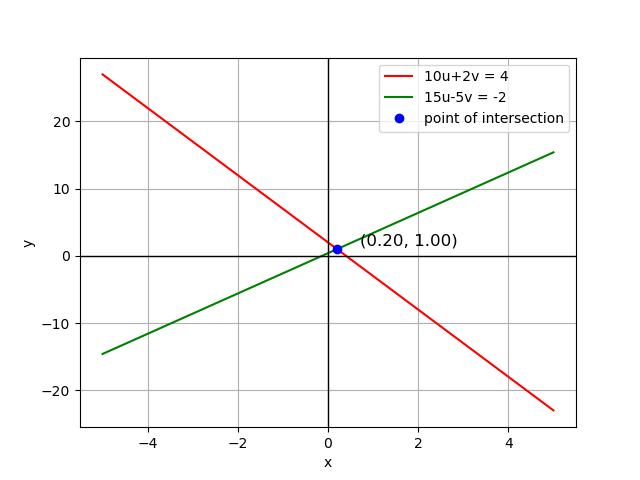
\includegraphics[width=1\columnwidth]{figs/fig.png}
   \caption{Intersection of two lines in $u-v$ space}
\end{figure}
\end{document}
